\documentclass[11pt,spanish]{article} % Idioma
\usepackage{babel}
\usepackage[T1]{fontenc}
\usepackage{textcomp, verbatim} % \begin{comment}
\usepackage[utf8]{inputenc} % Permite acentos

\usepackage{wrapfig} % Imagenes %\graphicspath{ {./imagenes/} }
\usepackage[left=2.75cm,top=2.5cm,right=2cm,bottom=2.5cm]{geometry} % Márgenes
\usepackage{amssymb, amsmath, amscd, amsfonts, amsthm, mathrsfs } % Símbolos matemáticos
\usepackage{cancel} % Cancelar expresiones
\usepackage{multirow, multicol, tabularx, booktabs, longtable} % Tablas
\usepackage{fancyhdr, fncychap} % Encabezados
\usepackage{algpseudocode, algorithmicx, algorithm} % Pseudo-código	
\usepackage{bbding} % Símbolos
\usepackage{enumitem} % Enumerados a), b), c)... usando \begin{enumerate}[label=\alph*)]
\usepackage{graphicx, xcolor, color, pstricks} % Gráficos --TikZ-- 
% http://www.texample.net/tikz/examples/
\usepackage[hidelinks]{hyperref}  % Enlaces
\usepackage{verbatim} % Comentarios largos \begin{comment}
\usepackage{rotating} % \begin{rotate}{30}
\usepackage[all]{xy} % Diagramas
\usepackage{xparse} % Entornos
\usepackage{listings}

\definecolor{codegreen}{rgb}{0,0.6,0}
\definecolor{codegray}{rgb}{0.5,0.5,0.5}
\definecolor{codepurple}{rgb}{0.58,0,0.82}
\definecolor{backcolour}{rgb}{0.95,0.95,0.92}

\lstdefinestyle{mystyle}{
	backgroundcolor=\color{backcolour},   
	commentstyle=\color{codegreen},
	keywordstyle=\color{magenta},
	numberstyle=\tiny\color{codegray},
	stringstyle=\color{codepurple},
	basicstyle=\footnotesize,
	breakatwhitespace=false,         
	breaklines=true,                 
	captionpos=b,                    
	keepspaces=true,                 
	numbers=left,                    
	numbersep=5pt,                  
	showspaces=false,                
	showstringspaces=false,
	showtabs=false,                  
	tabsize=2
}
\lstset{style=mystyle}


% Comandos
\newcommand{\docdate}{}
\newcommand{\subject}{}
\newcommand{\docauthor}{Rubén Morales Pérez}
\newcommand{\docemail}{srmorales@correo.ugr.es}

\newcommand{\N}{\mathbb{N}}
\newcommand{\Q}{\mathbb{Q}}
\newcommand{\C}{\mathbb{C}}
\newcommand{\R}{\mathbb{R}}
\newcommand{\Z}{\mathbb{Z}}


\linespread{1.1}                  % Espacio entre líneas.
\setlength\parindent{0pt}         % Indentación para párrafo.

\title{Prácticas Fundamentos de Redes\\ Chat}
\author{Rubén Morales Pérez\\
		Francisco Javier Morales Piqueras}
\date{\today}

% % % % % % % % % % % % % % % % % % % % % % % % % % % % % % % % %
%					 Inicio del documento
% % % % % % % % % % % % % % % % % % % % % % % % % % % % % % % % %
\begin{document}

\maketitle
\tableofcontents % Generando el indice
\newpage
\setlength\parindent{0pt} % Quitamos la sangría


\section{Introducción}
En esta práctica crearemos un chat multiusuario usando el paradigma cliente-servidor.
El servidor será un proceso alojado en alguno de los ordenadores de la comunicación.
El servidor será el encargado de mandar el mensaje a los usuarios implicados en la comunicación, y solamente a ellos.
La práctica será realizada en \textit{JAVA}.

La estructura del programa es la siguiente.

\begin{figure}[h]
	\centering
	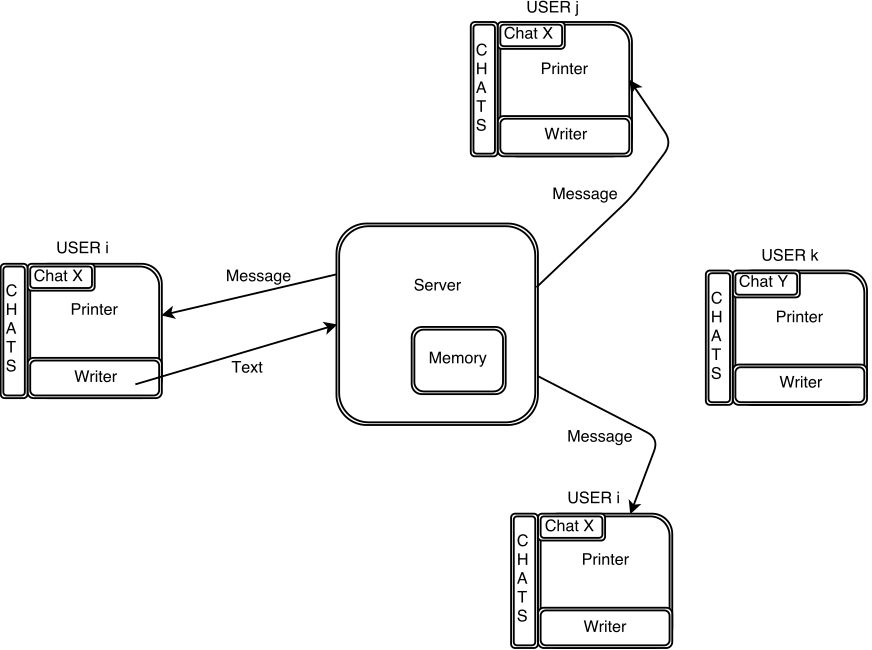
\includegraphics[width=0.9\textwidth]{./Imagenes/chat.png}
\end{figure}
\section{Servidor}
El servidor será una clase \textbf{Server} que estará continuamente recibiendo y mandando mensajes.
Guardará los sockets necesarios para la comunicación.
El servidor tiene una serie de archivos guardados para su organización.

\vspace{0.1cm}

\begin{figure}[H]
	\centering
	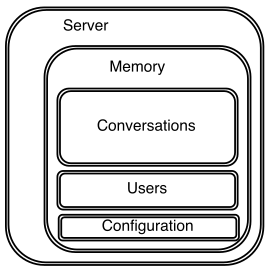
\includegraphics[width=0.45\textwidth]{./Imagenes/server.png}
\end{figure}
\section{Usuario}
\subsection{Representación}
Un usuario quedará identificado por su \textit{idUser}, los usuarios se guardarán en una carpeta especial con ficheros como el siguiente.
\lstinputlisting[caption=0.usr]{../.chatConfig/users/0.usr}
La estructura del fichero es la siguiente
\begin{itemize}
	\item Identificador de usuario
	\item Nombre de usuario
	\item Contraseña
	\item Grupos a los que pertenece
\end{itemize}

Esta configuración permite tener un chat con nosotros mismos.
Existirán funciones para cargar y guardar usuarios en ficheros.


\subsection{Mensajes}
Cada usuario tiene una instancia de la clase \textit{Printer} que recibirá y mostrará los mensajes.
Los mensajes tienen un identificador del grupo al que pertenecen, del usuario que los envía y un identificador del mensaje.
Estos tres parámetros nos permitirán identificar de forma única cada mensaje.

\begin{figure}[H]
	\centering
	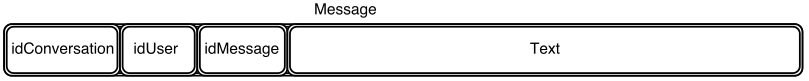
\includegraphics[width=0.8\textwidth]{./Imagenes/message.png}
\end{figure}

Un fichero de conversación será una sucesión de mensajes, como muestra el siguiente ejemplo.

\lstinputlisting[caption=example.chat]{../.chatConfig/conversations/example.chat}

Los números al inicio son el identificador de conversación, el del usuario que manda el mensaje y el identificador de su mensaje.
Estos tres números en conjunto formarán el identificador de cada mensaje.
\section{Configuración}
La configuración del chat la manejaremos con una clase llamada \textit{Config}.
En la clase tendremos los directorios con ruta absoluta de las diferentes carpetas necesarias.
Habrá variables para controlar cuántos usuarios y conversaciones tenemos registrados en el sistema, y los puertos usados para las comunicaciones.
También tendremos guardadas las extensiones con las que guardaremos los ficheros de usuarios y conversaciones.

Al inicializar una instancia de la clase \textbf{Config} se crearán las carpetas necesarias para el manejo de usuarios y conversaciones.
Tendremos funciones para guardar la configuración actual y para acceder al fichero de cada conversación o usuario. También podremos comprobar si existe un usuario o conversación.


%%%%%%%%%%%%%%%%%%%%%%%%%%%%%%%%%%%%%%%%%%%%%%%%%%%%%%%%%%%%%%%%%%%%%%%%%%%%%%%%%%

% % % % % % % % % % % % % % % % % % % % % % % % % % % % % % % % %
%					 Bibliografía
% % % % % % % % % % % % % % % % % % % % % % % % % % % % % % % % %

\end{document}
